\documentclass[../../DD.tex]{subfiles}
\begin{document}
\section{Kinds of Topic \label{sect:2.1}}
	\subsection{Musical Instrument}
		Musical Instrument page contains the name, the description and the history of the instrument itself. If there is a course of that instrument, a link to the relative course shows up. There might be very simple instruments that have no course (e.g. Triccheballacche is a percussion instrument with a single sound). Related instruments are other musical instruments that are from the same region or of the same instrument type.
		\newline
		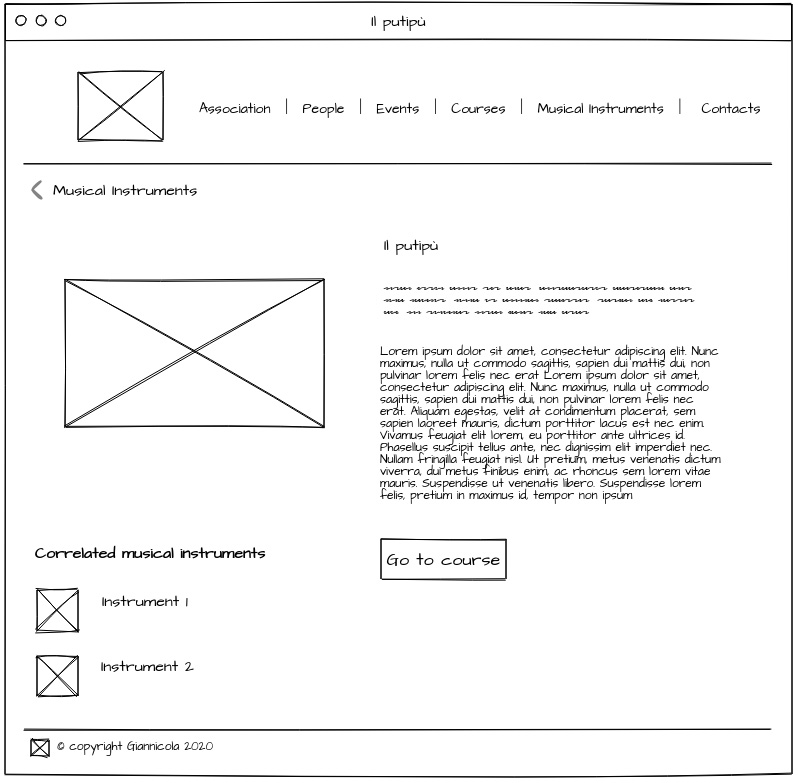
\includegraphics[width=\textwidth,height=\textheight,keepaspectratio]{Wireframes/KOTMusicalInstrument.jpg}

	\subsection{Course}
		Single course page has two main section: the first one represents information about the course, with its description and a detail section containing the days and the room of the lessons; below, there are links to the instrument teached (if it does exists, there might be courses with no instrument like singing ones) and to the teachers pages.  
		\newline
		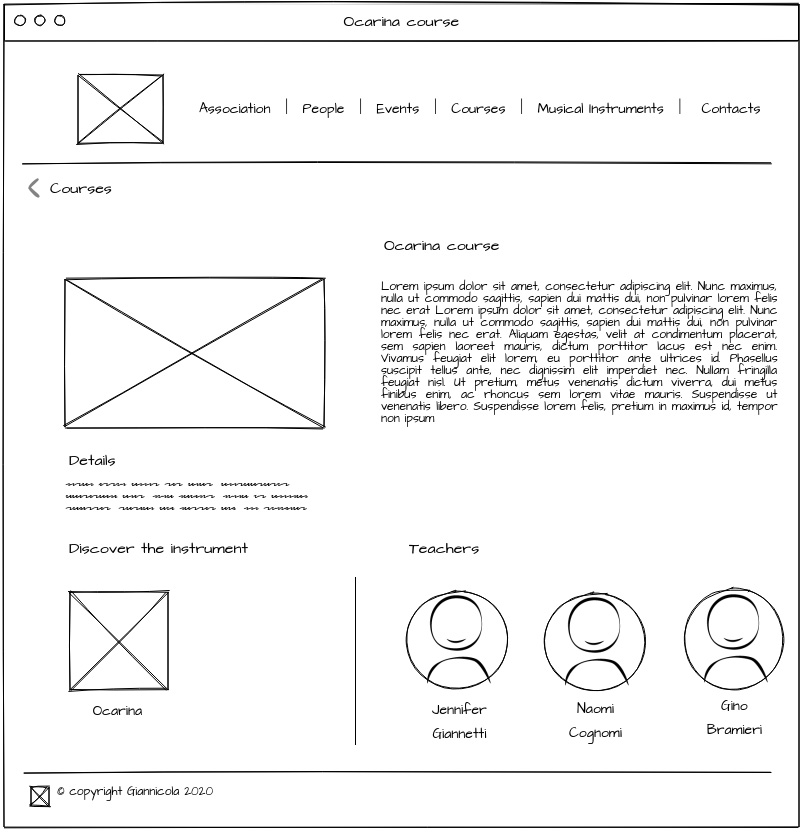
\includegraphics[width=\textwidth,height=\textheight,keepaspectratio]{Wireframes/KOTCourse.jpg}

	\subsection{Person}
		Person represents the page of a person that is involved in the association. Even if most of them are teachers, this is not necessarily true. The page contains the name, a profile image and a biography of the person, and a contact section, with email and phone number. If this person is a teacher, the page contains also links to her courses.
		\newline
		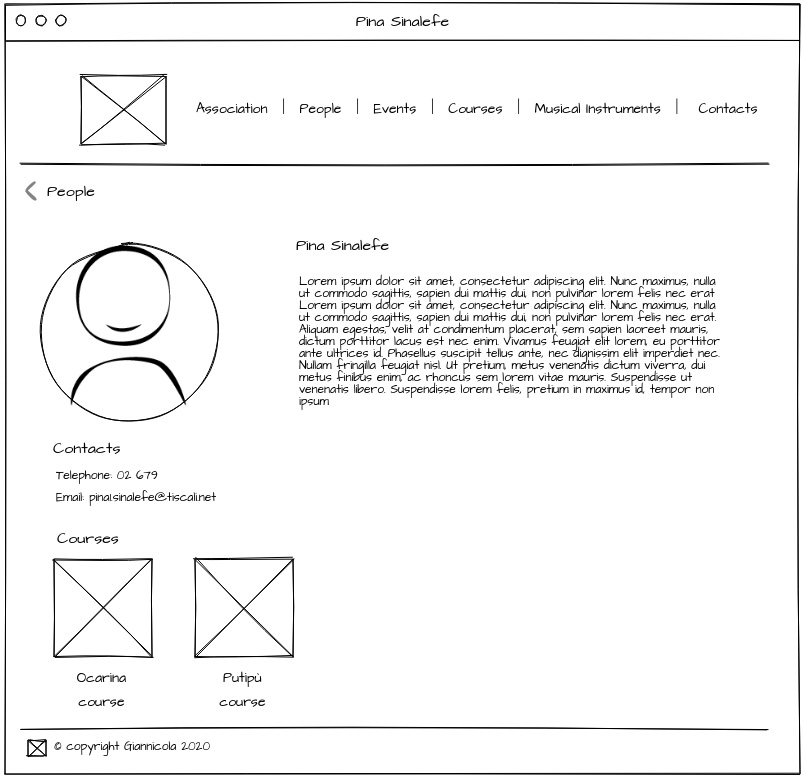
\includegraphics[width=\textwidth,height=\textheight,keepaspectratio]{Wireframes/KOTPerson.jpg}

	\subsection{Event}
		Event page is where the user can find all the information about a single event. The title of the event is shown with an image and a description. A details section contains information about time and date of the event. Below there are the courses presented during the event (if there are some) and a link to the organizer's personal page, where her contacts and biography are.
		\newline
		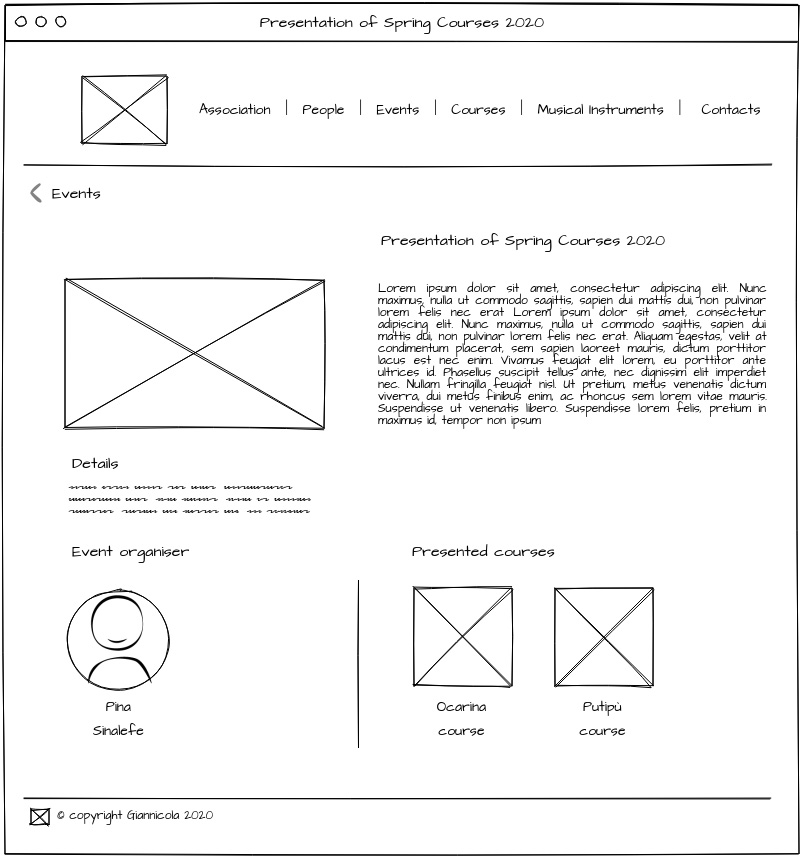
\includegraphics[width=\textwidth,height=\textheight,keepaspectratio]{Wireframes/KOTEvent.jpg}
\end{document}
